\section{Zastosowane wzorce projektowe}
\label{sec:patterns}
Wzorce projektowe zostały stworzone po to, aby uschematyzować proces rozwiązywania powstałych problemów projektowych w tworzeniu, komunikacji i organizacji struktury kodu. Skategoryzowano je i opisano w publikacji Design Patterns: Elements of Reusable Object-Oriented Software\footnote{Publikacja wydana w 1995 r., autorstwa tzw. Bandy Czworga: E.Gamma, R.Helm, R. Johnson, J. Ulisside}.

Budowa języka Ruby oraz framework Ruby on Rails zachęca programistów do korzystania ze znanych wzorców projektowych. Dzięki wykorzystaniu tych technologii mamy możliwość korzystania z zaimplementowanych wzorców w samym szkielecie aplikacji.
  \subsection{MVC}
  \index{MVC}
   Model-Widok-Kontroler(\emph{Model-View-Controller}), wzorzec projektowy określający schemat całej aplikacji. Jest on domyślnie wbudowany w Ruby on Rails. Jego zadaniem jest podział struktury aplikacji na: logikę, opis interfejsu i komunikację połączoną z zarządzaniem.
   MVC zbudowany jest z pomniejszych wzorców projektowych.
    \begin{itemize}
      \item \textbf {Model} \\
      Model odpowiada za logikę aplikacji, zarządza dostępem do bazy danych.
      Poprzez dziedziczenie po klasie ActiveRecord implementuje wzorce takie jak: Budowniczy\footnote{\emph{z ang. Builder pattern}, wzorzec oddziela reprezentację obiektu od procesów jego tworzenia. \cite{ruby_patterns}}, Obserwator\footnote{\emph{z ang. Observer pattern}, zadaniem wzorca projektowego Observer jest śledzenie zmian występujących w obiektach obserwowanych i informowanie o nich obiektu nadrzędnego - obserwatora. \cite{ruby_patterns}}, czy wzorzec Poleceń\footnote{\emph{z ang. Command pattern}, reprezentuje on zapytania jako obiekty, zwiększając tym samym elastyczność działania\cite{ruby_patterns}}.

      \item \textbf {Widok} \\
      Tworzy interfejs użytkownika zapewniając prezentację danych. Łączy ze sobą wzorce takie jak: wzorzec Kompozycji\footnote{z ang. Composite pattern, grupuje on obiekty w jeden aby móc wykonywać na nich operacje w ten sam sposób. \cite{ruby_patterns}}, wzorzec Strategii i wzorzec Obserwatora.

      \item \textbf {Kontroler} \\
      Odpowiada za obsługę żądań przychodzących od użytkownika, poprzez delegowanie zadań. Jest pośrednikiem pomiędzy logiką biznesową (\emph{Model}), a warstwą prezentacji danych (\emph{View}). W swoim działaniu posługuje się wzorcem Strategii\footnote{ \emph{z ang. Strategy pattern}, wzorzec ma za zadanie dostarczyć do obiektu kontekstowego, inne obiekty potrafiące wykonać określony algorytm. \cite{ruby_patterns}}.
    \end{itemize}

    Rysunek nr \ref{fig:model_mvc} przedstawia sposób komunikacji poszczególnych warstw modelu MVC:
    \begin{figure}[h]
      \centering
      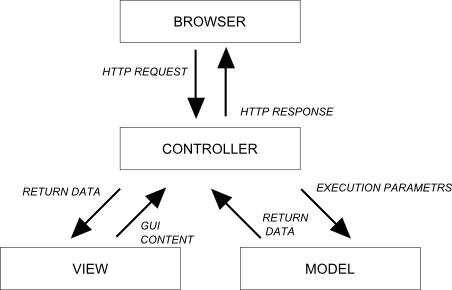
\includegraphics[scale=0.87]{images/mvc_model.png}
      \caption{Schemat MVC}
      \label{fig:model_mvc}
    \end{figure}
  \clearpage
  \subsection{Iteraktor}
  \index{Interaktor}
  Interaktor\cite{interactors}(\emph{Interactor}), inaczej nazywany Obiektem pomocniczym (\emph{Service Object}).
  Jest wzorcem projektowym, który ma za cel wykonanie określonych zadań wydelegowanych z warstwy kontrolera w modelu MVC. Taki mechanizm upraszcza strukturę kodu i ułatwia stosowanie się do zasad: Prosty Kontroler i Model (\emph{Skiny Controllers and Models}), \index{SOLID}SOLID.
  Interactor stanowi warstwę pośredniczącą pomiędzy przekazywaniem danych między kontrolerem a modelem.
  Dzięki temu uzyskuje się większą przejrzystość zarówno modelu jak i kontrolera. Przeniesiona zostaje odpowiedzialność za walidację. Testowanie aplikacji jest stosunkowo szybkie i łatwe. Każde zadanie wykonywane przez Interaktor testowane jest w izolacji\footnote{Testowany jest konkretny obiekt, bez względu na jego relacje z innymi obiektami.}.

  W poniższym przykładzie przedstawiliśmy wykorzystanie wzorca porjektowego Interaktor zastosowanego do rejestracji użytkowników do newslettera:\\
  \begin{code}
  \lstinputlisting[language = Ruby]{../meetspace/app/interactions/subscriber_registration.rb}
\end{code}

